\subsection{Conceptual Genesis: Desire and Unsettling}

The persona of Sun Ra, the enigmatic jazz bandleader, composer, and cosmic philosopher, claimed to have arrived on Earth from Saturn, a mythology elaborated most famously in the 1974 film \emph{Space is the Place}. This Afrofuturist origin story positions Sun Ra as an interstellar traveler, raising a speculative question that grounds this work: on his journey from Saturn to Earth, did he fear entering cryosleep? The question is both playful and serious, opening onto larger investigations of how Black bodies are depicted in states of suspension, transition, and passage through space-time.

\begin{figure}[H]
	\centering
	% Top row: 2 larger images
	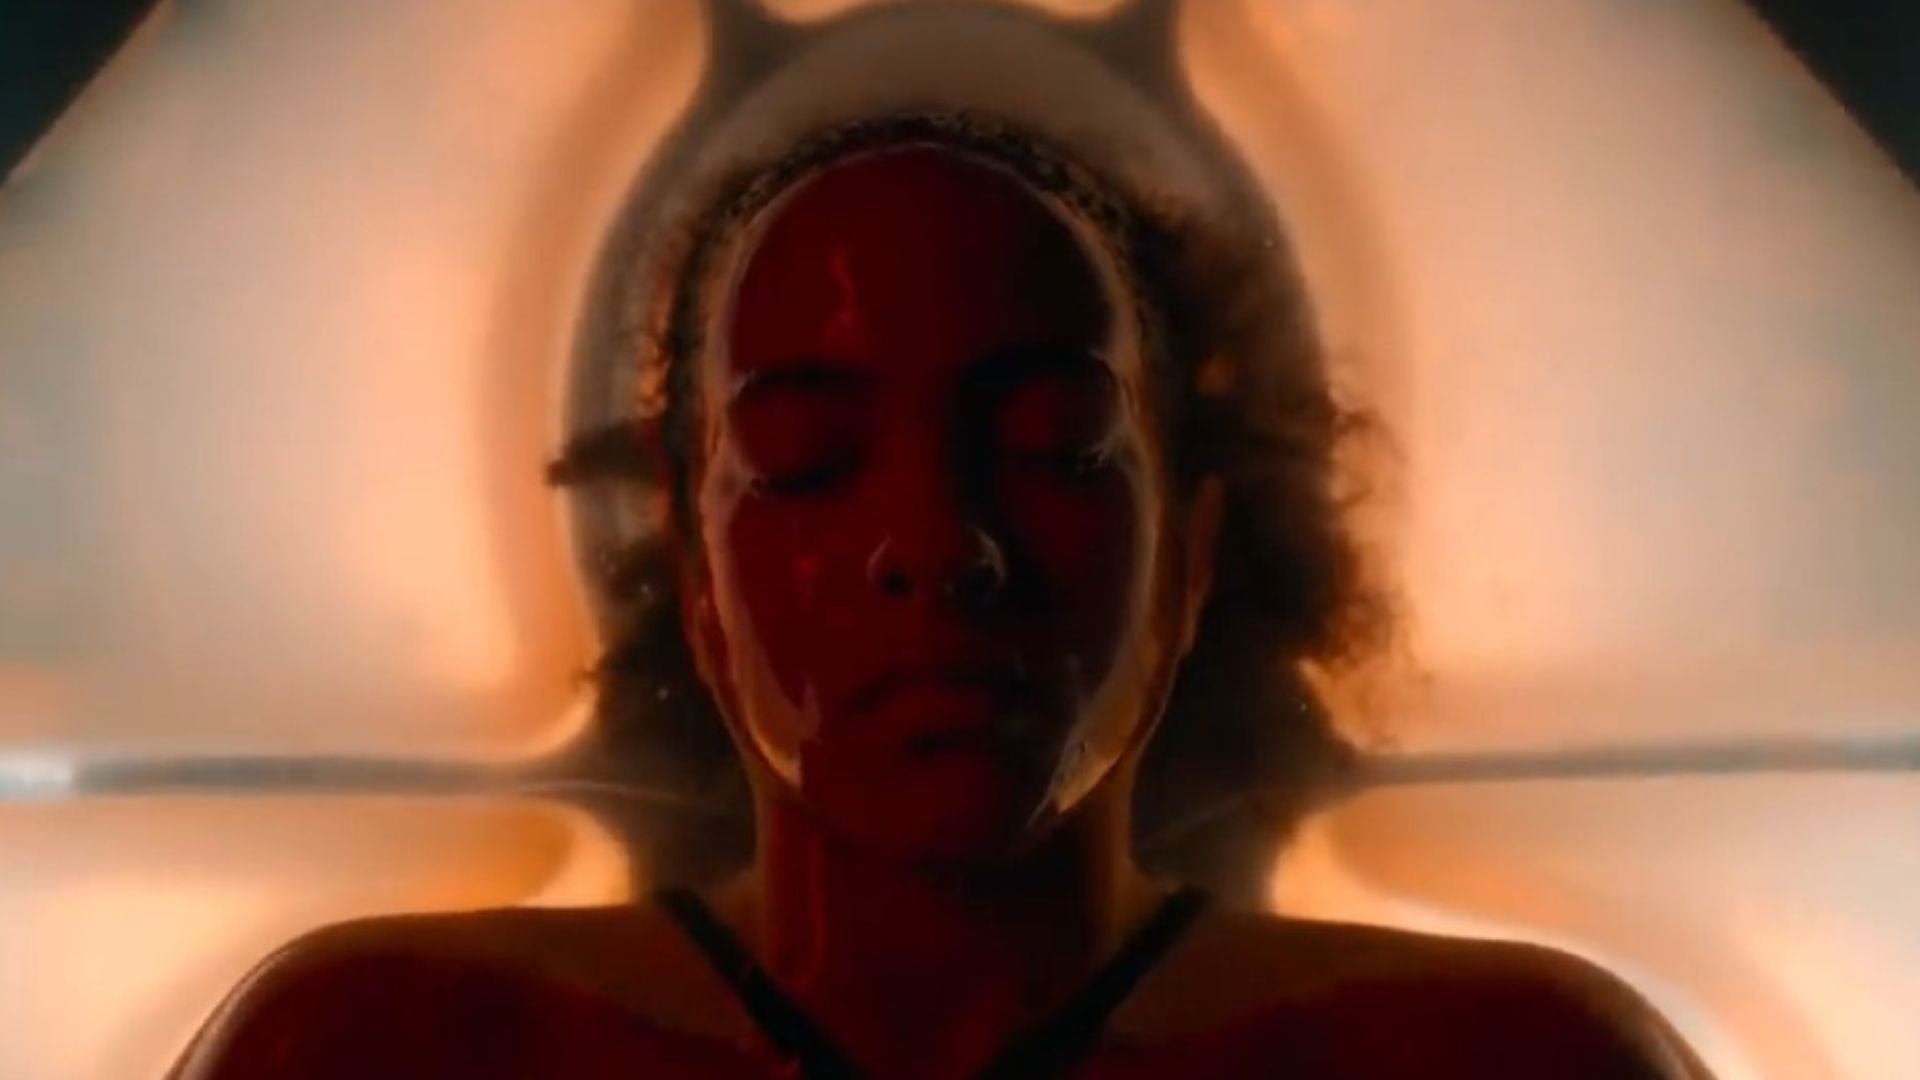
\includegraphics[width=0.45\textwidth]{assets/figures/gaal_cryosleep.jpg}\hfill
	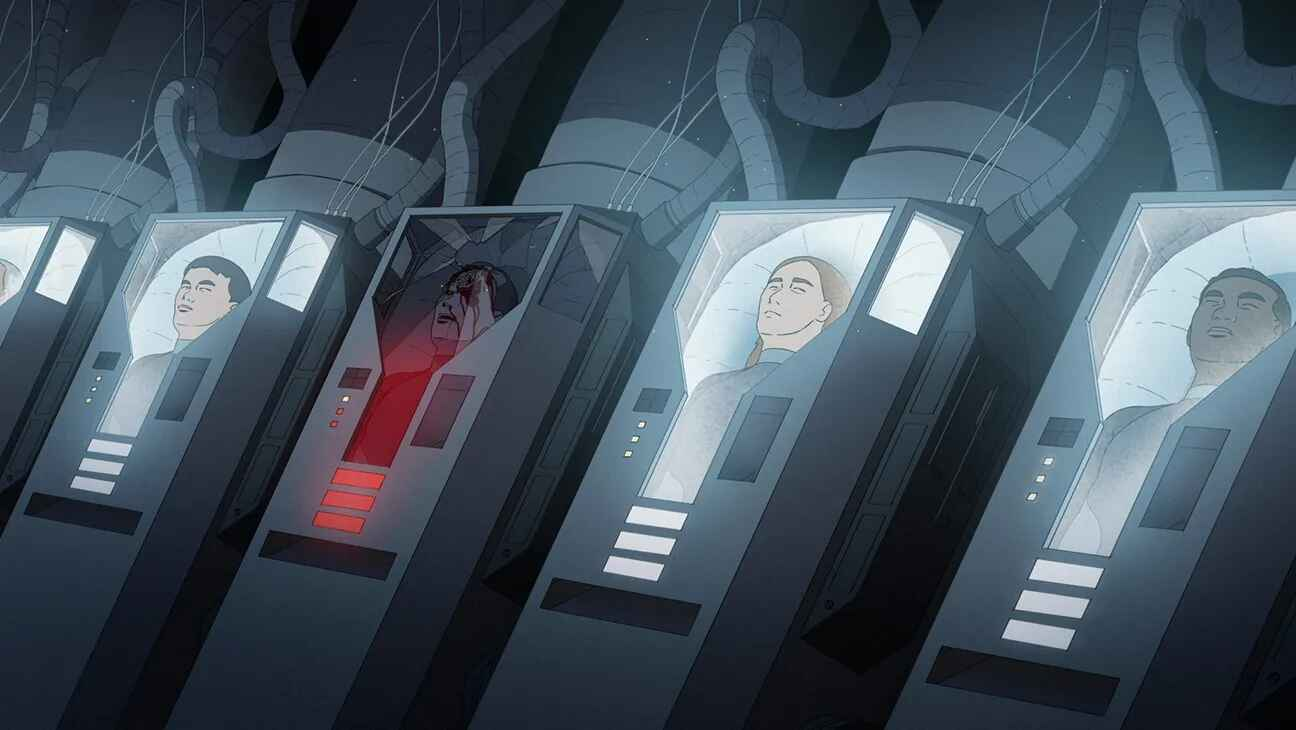
\includegraphics[width=0.45\textwidth]{assets/figures/scavengers-reign_0.jpg}
	
	\vspace{0.5em}
	
	% Bottom row: 3 smaller images
	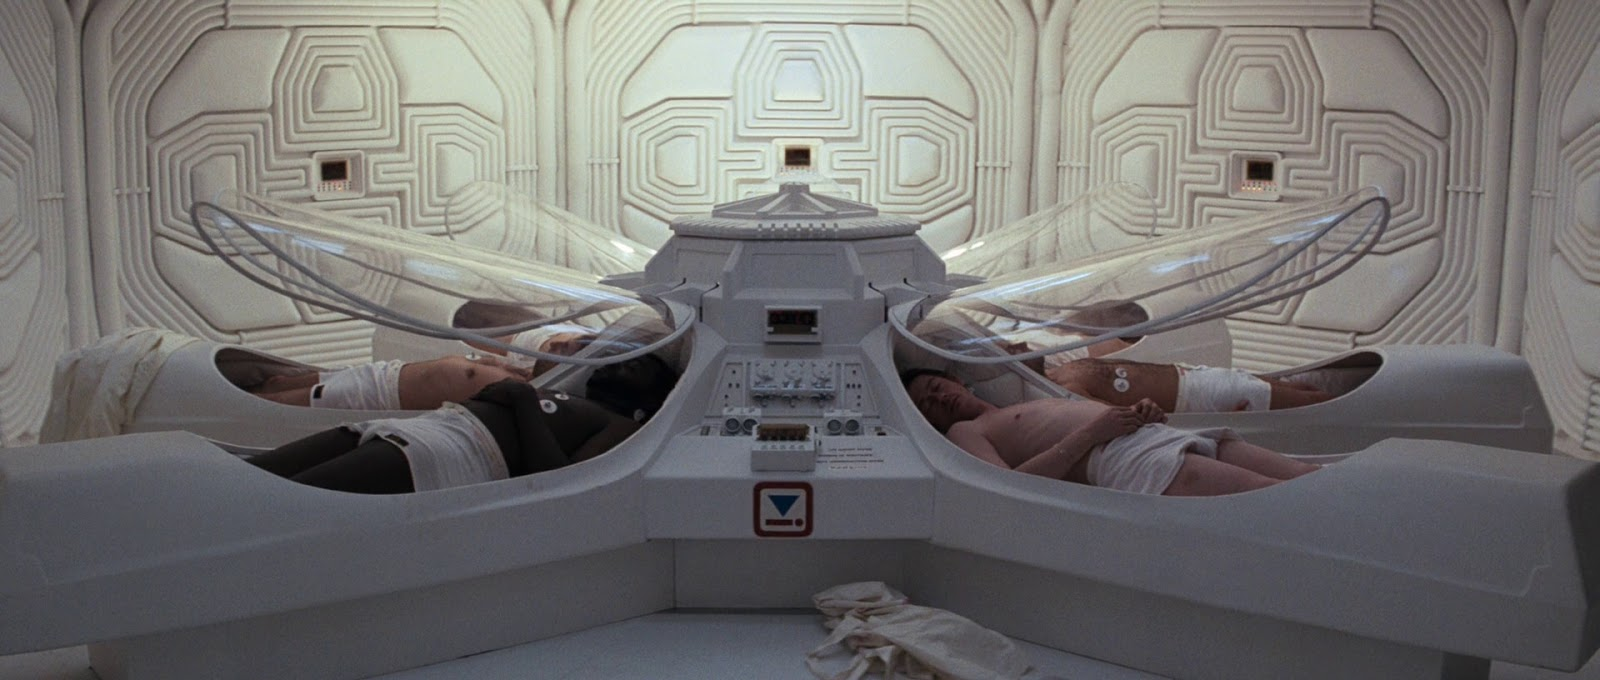
\includegraphics[width=0.31\textwidth]{assets/figures/alien_hypersleep_chamber.jpg}\hfill
	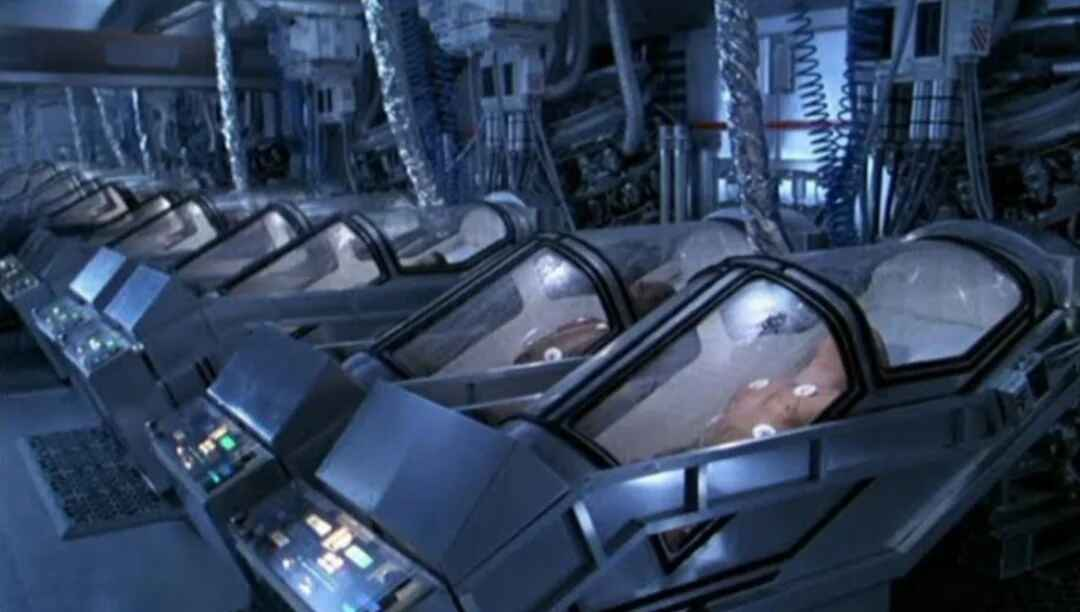
\includegraphics[width=0.31\textwidth]{assets/figures/aliens-hypersleep.jpg}\hfill
	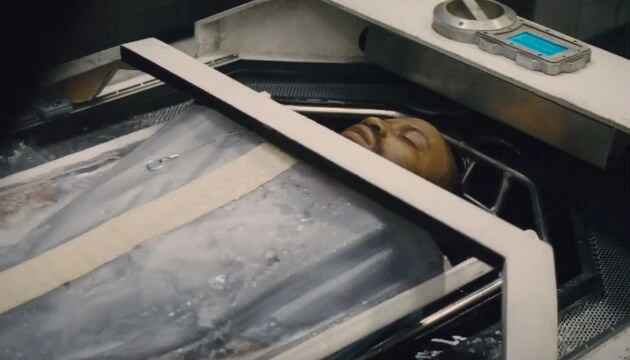
\includegraphics[width=0.31\textwidth]{assets/figures/Romilly_sleeptosaturn.jpg}
	
	\caption{Black bodies in suspension across science fiction narratives: \emph{Foundation} \parencite{GRAVES_2021}, \emph{Scavengers Reign} \parencites{BROOKE_2023} (top); \emph{Alien} \parencites{SCOTT_1979}, \emph{Aliens} \parencites{CAMERON_1986}, \emph{Interstellar} \parencites{NOLAN_2014} (bottom). These visual tropes frequently depict Black bodies with water, stasis, and passage through space-time, evoking both speculative futures and the historical trauma of the Middle Passage.}
	\label{fig:cryosleep-collage}
\end{figure}

Science fiction and fantasy narratives frequently depict cryosleep and stasis through imagery of bodies submerged in fluid (or otherwise being "frozen" is a state of suspended animation), from the amniotic pods of \emph{The Alien Franchise} to the deep space faring cryo-pods of \emph{Foundation}, and countless other examples. For Black bodies specifically, this visual motif carries additional historical resonance: the forced passage of the Middle Passage, bodies packed into ship holds, the Atlantic Ocean as both a grave and archive. Water and fluid become sites where historical fact and speculative fiction converge, where the transpiration of Black bodies across space-time is simultaneously remembered and reimagined. This work investigates that convergence through the literal materiality of water, sediment, and dissolution.

\begin{figure}[H]
	\centering
	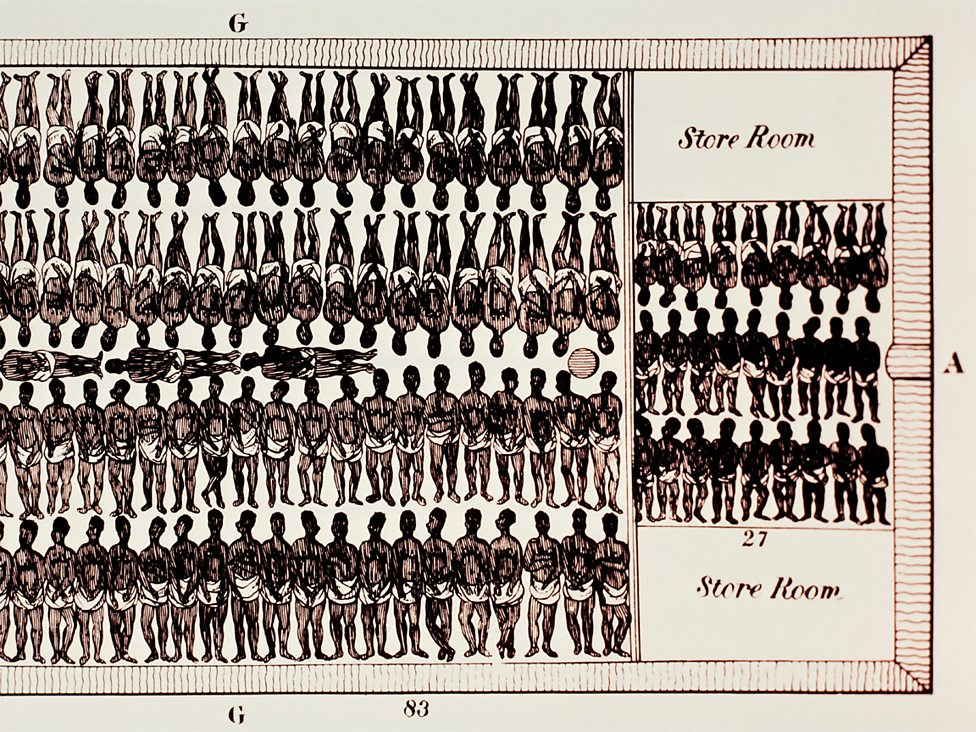
\includegraphics[width=0.7\textwidth]{assets/figures/middle-passage-shiphold.jpg}
	\caption{Depiction of enslaved Africans in the hold of a slave ship bound for the middle passage. The method of "tight packing" often used meant placing as many bodies as possible in the hold for maximum profit, but also resulted in the loss of more life due to the cramped, unsafe conditions. \parencites{BBC_2025}}
	\label{fig:middle-passage}
\end{figure}

\subsection{Material and Sonic Form: Signal and Remixing}

\begin{figure}[H]
	\centering
	
	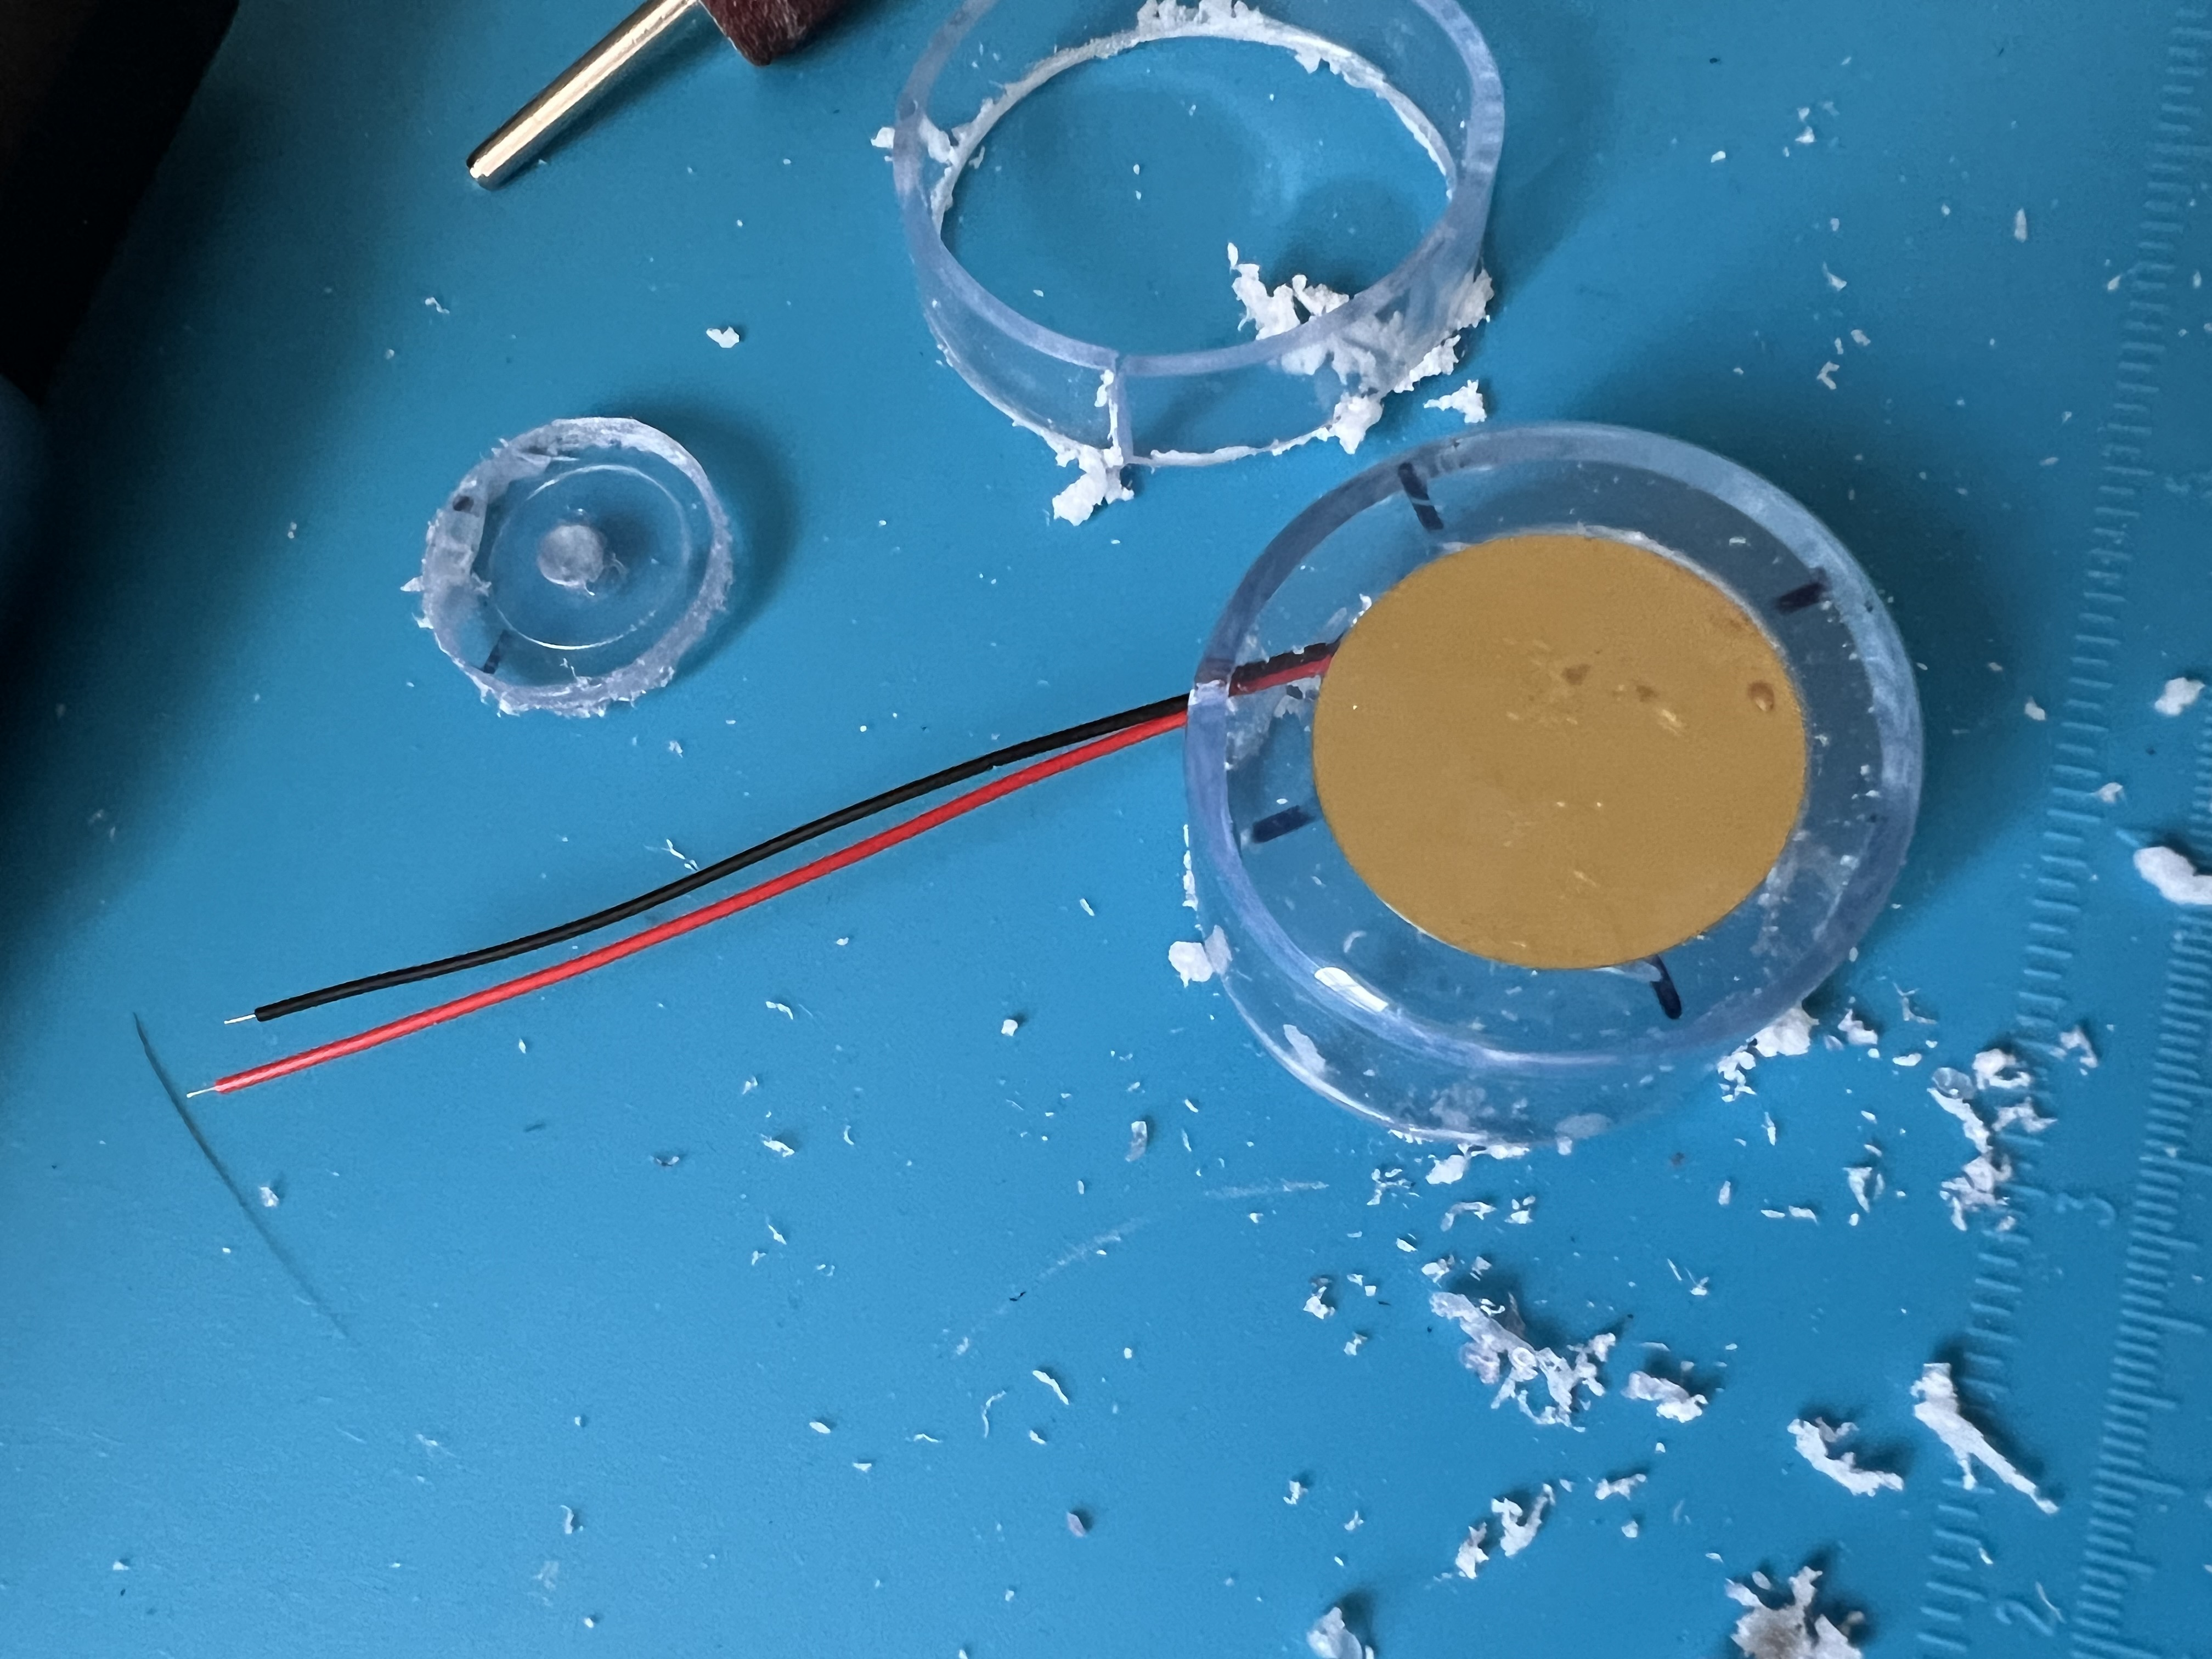
\includegraphics[width=0.31\textwidth]{assets/figures/IMG_6583.jpeg}\hfill
	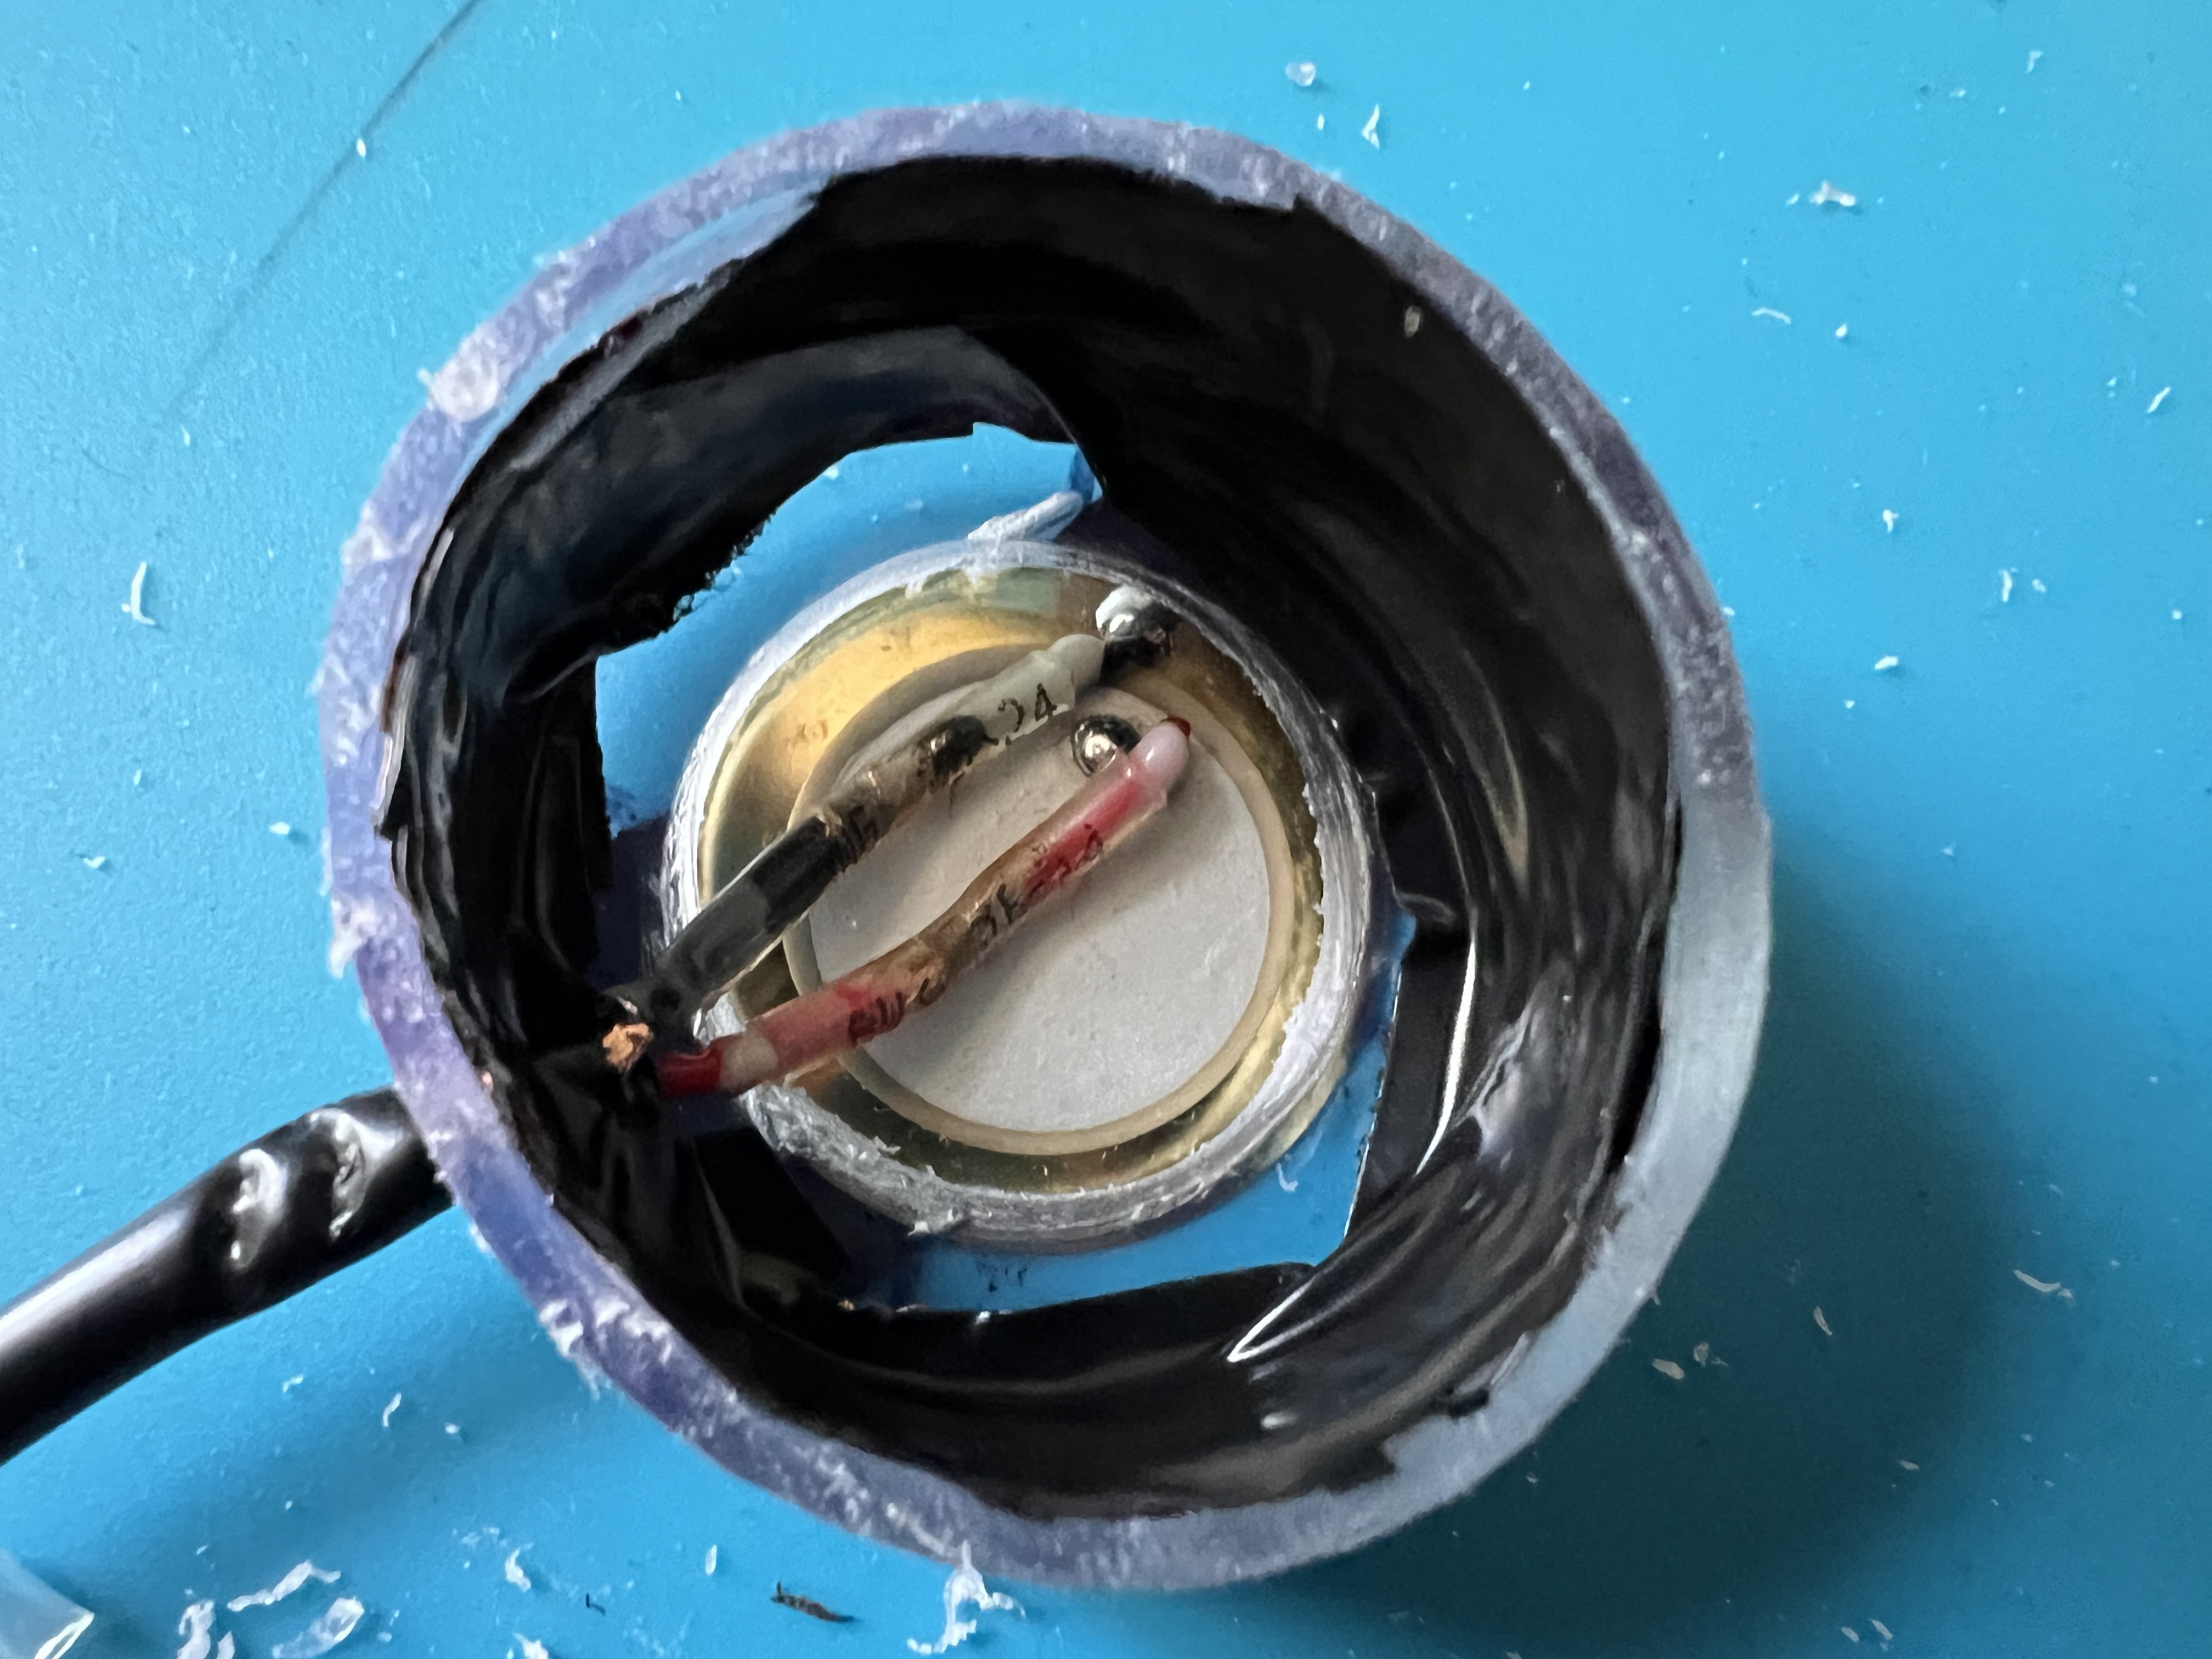
\includegraphics[width=0.31\textwidth]{assets/figures/IMG_6586.jpeg}\hfill
	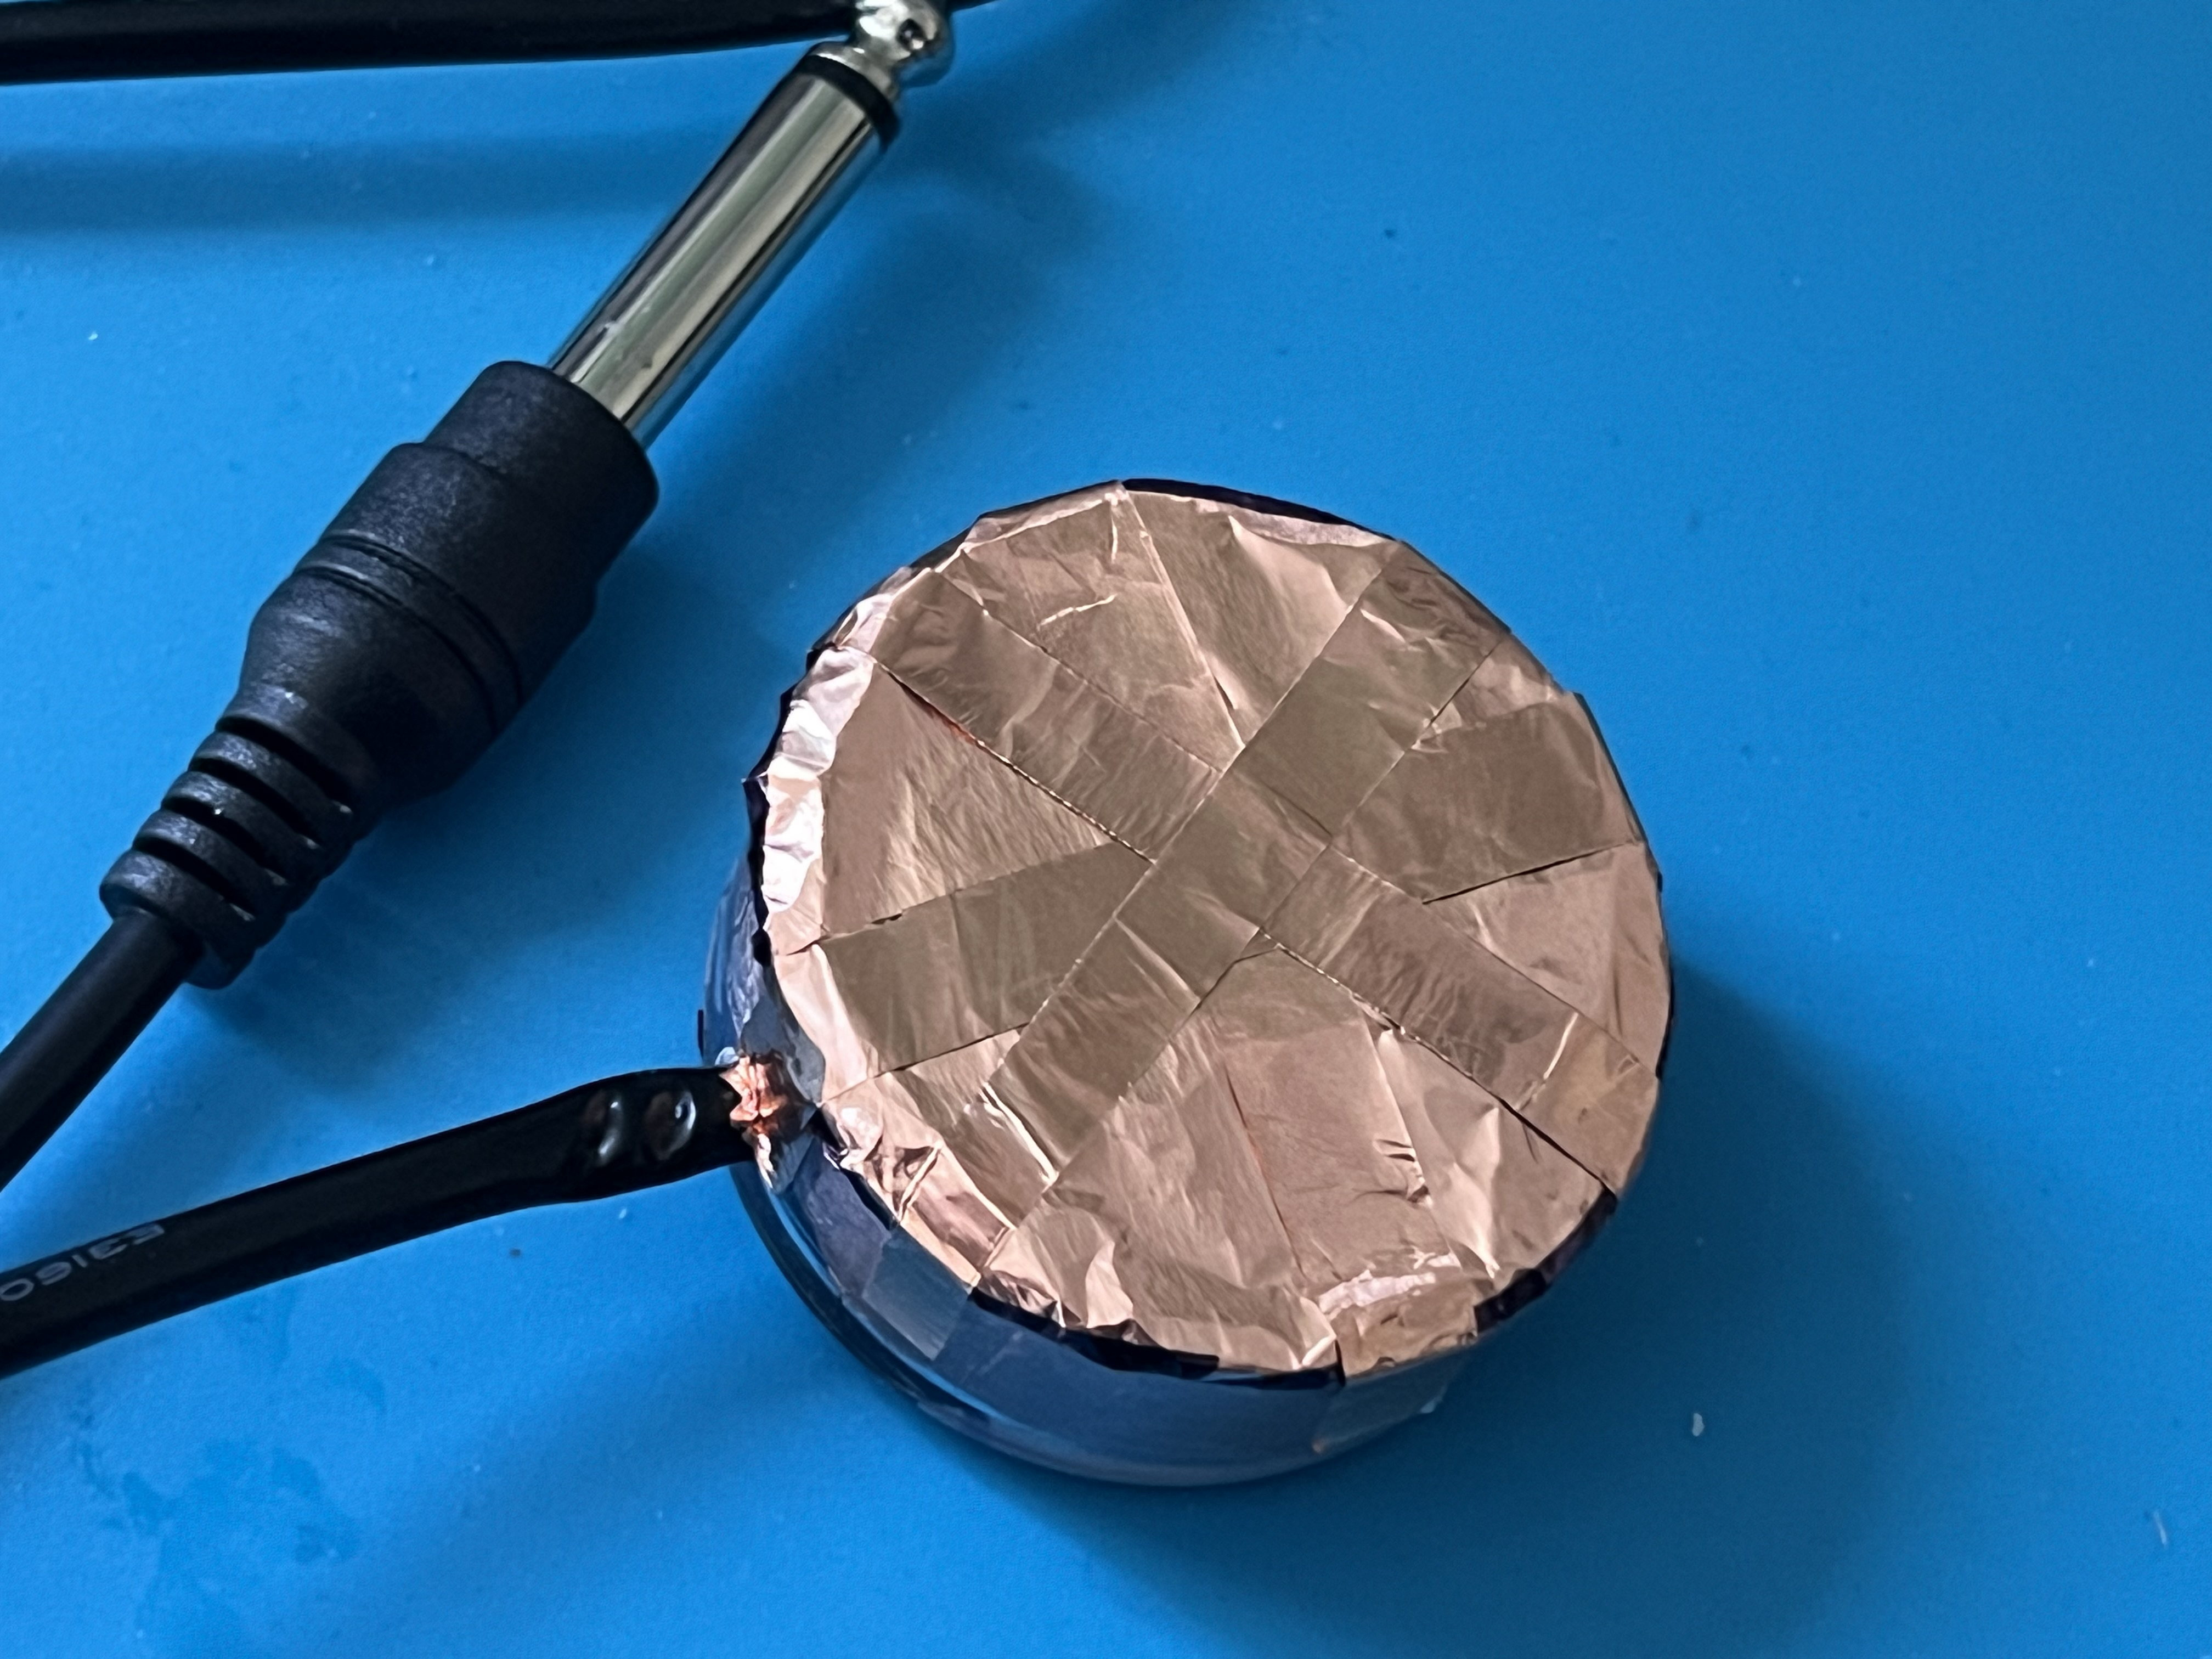
\includegraphics[width=0.31\textwidth]{assets/figures/IMG_6596.jpeg}\hfill
	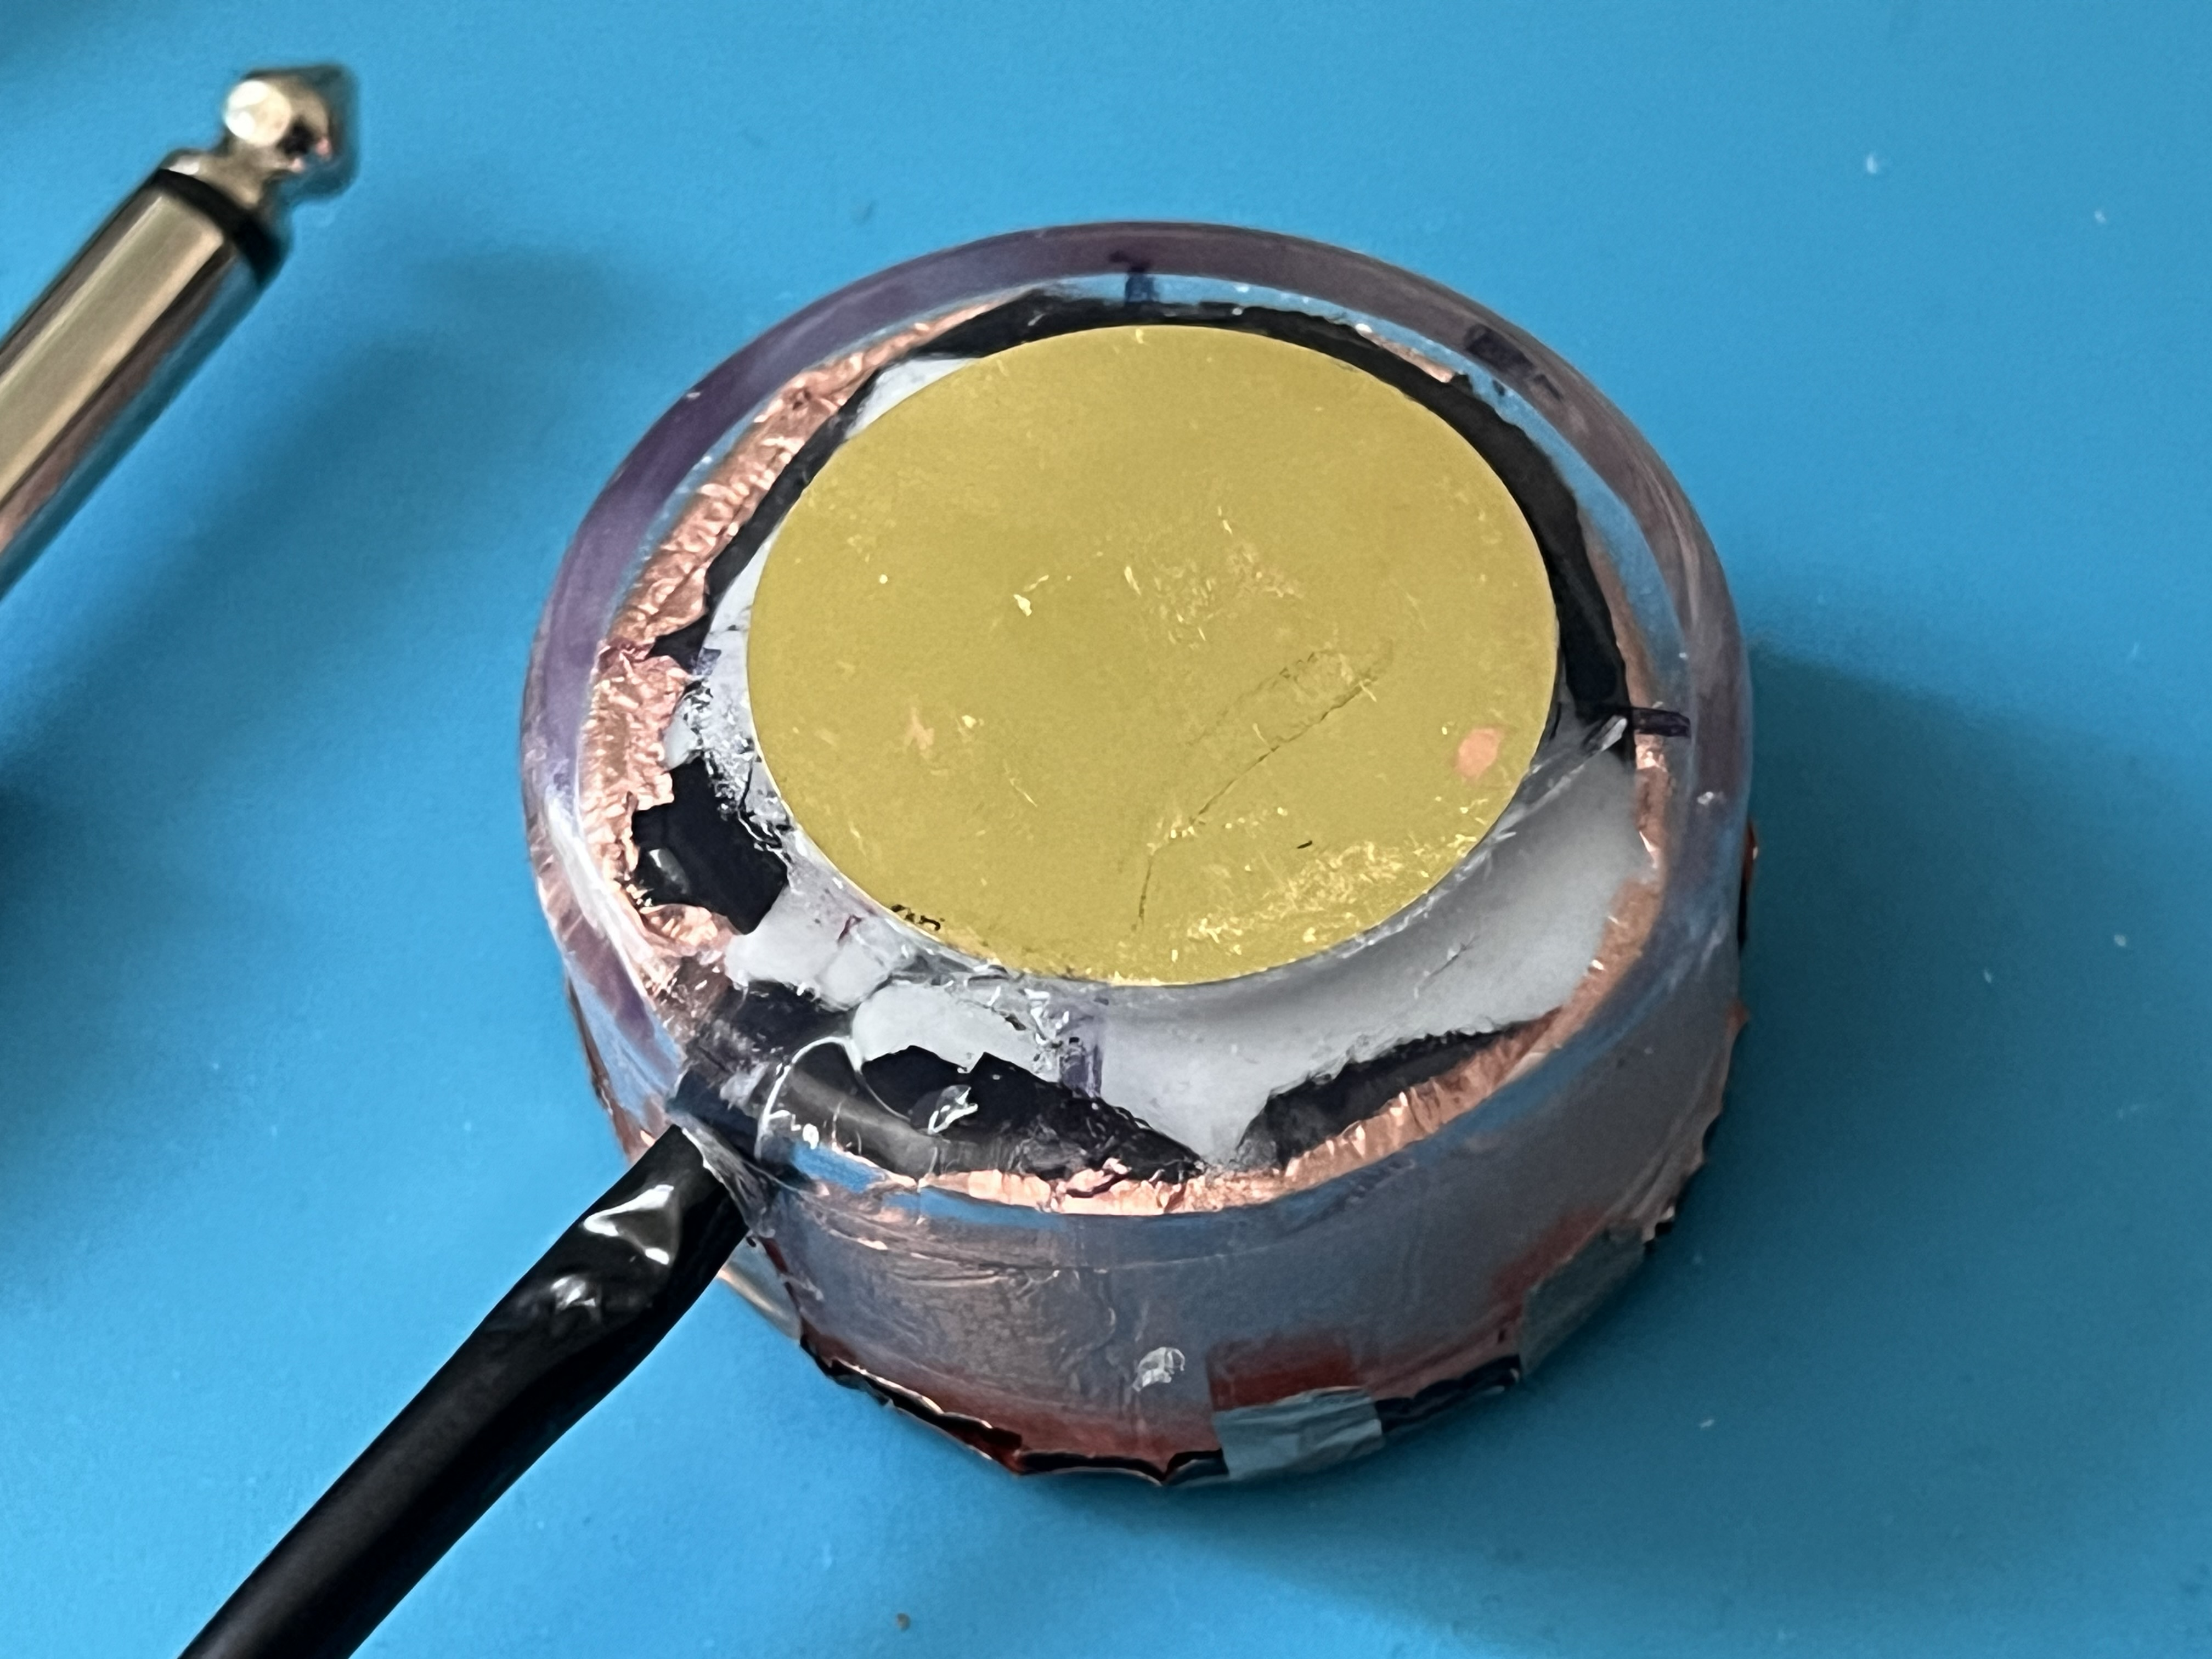
\includegraphics[width=0.31\textwidth]{assets/figures/IMG_6597.jpeg}\hfill
	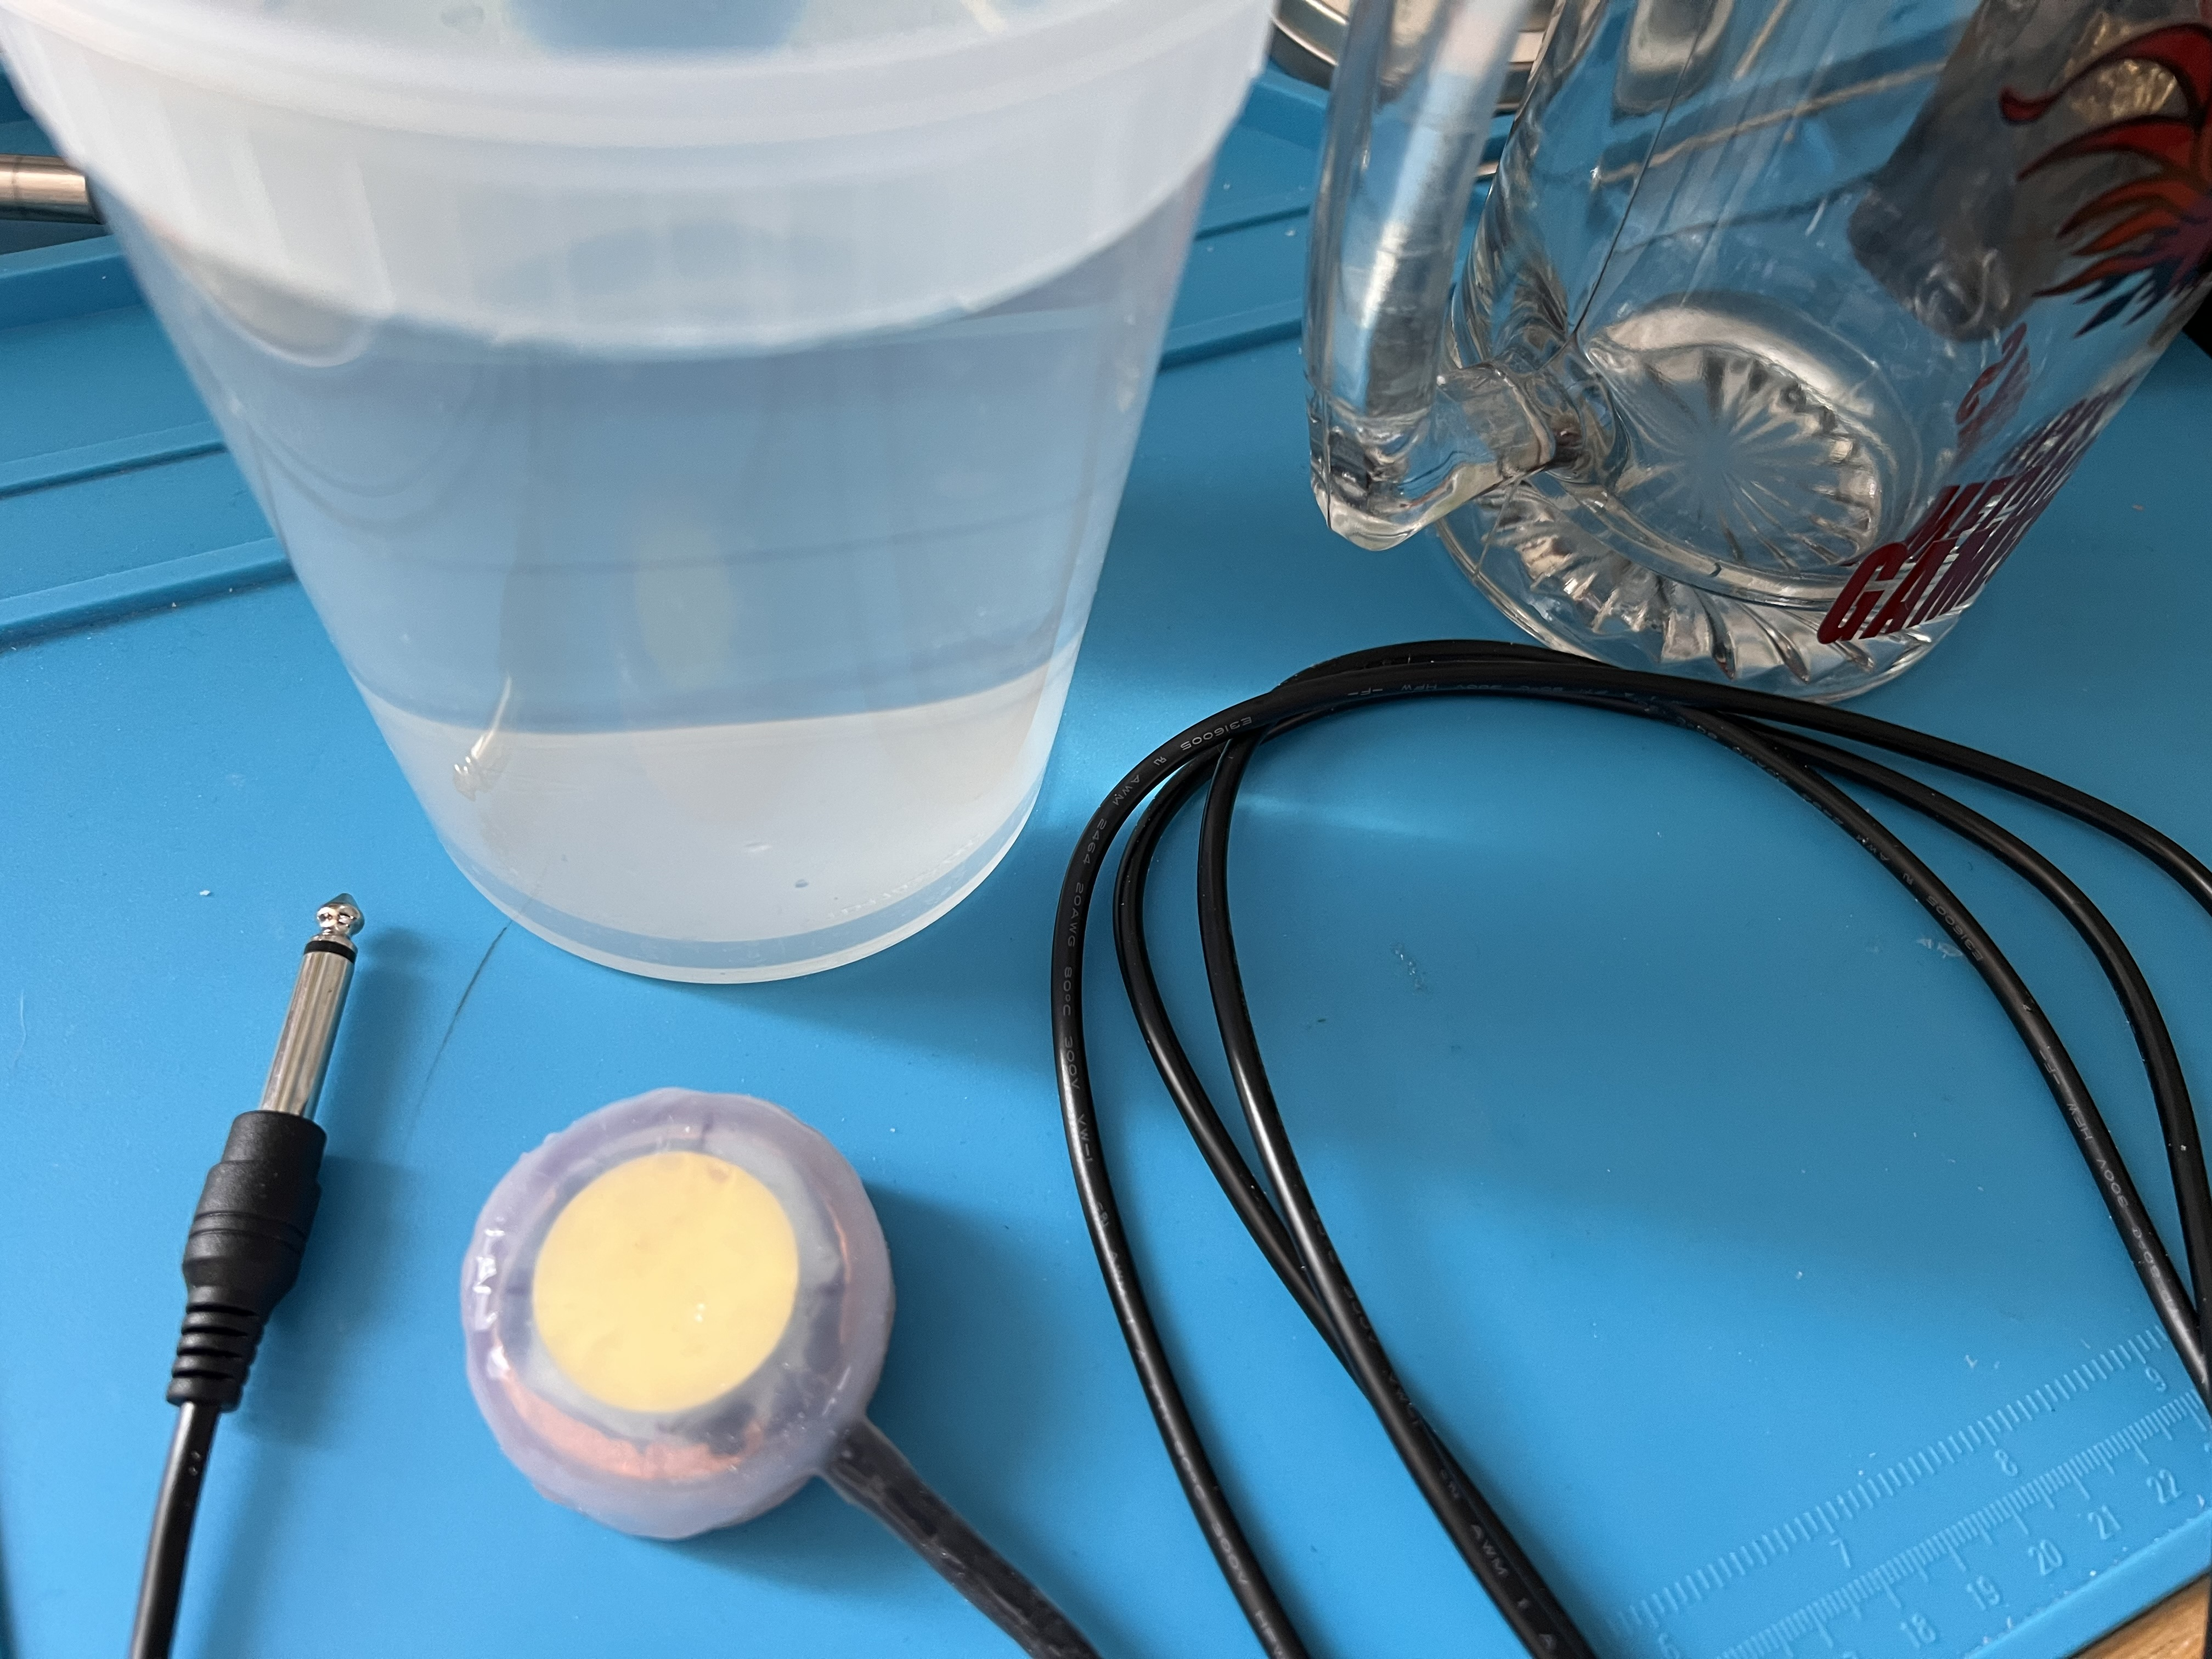
\includegraphics[width=0.31\textwidth]{assets/figures/IMG_6605.jpeg}\hfill
	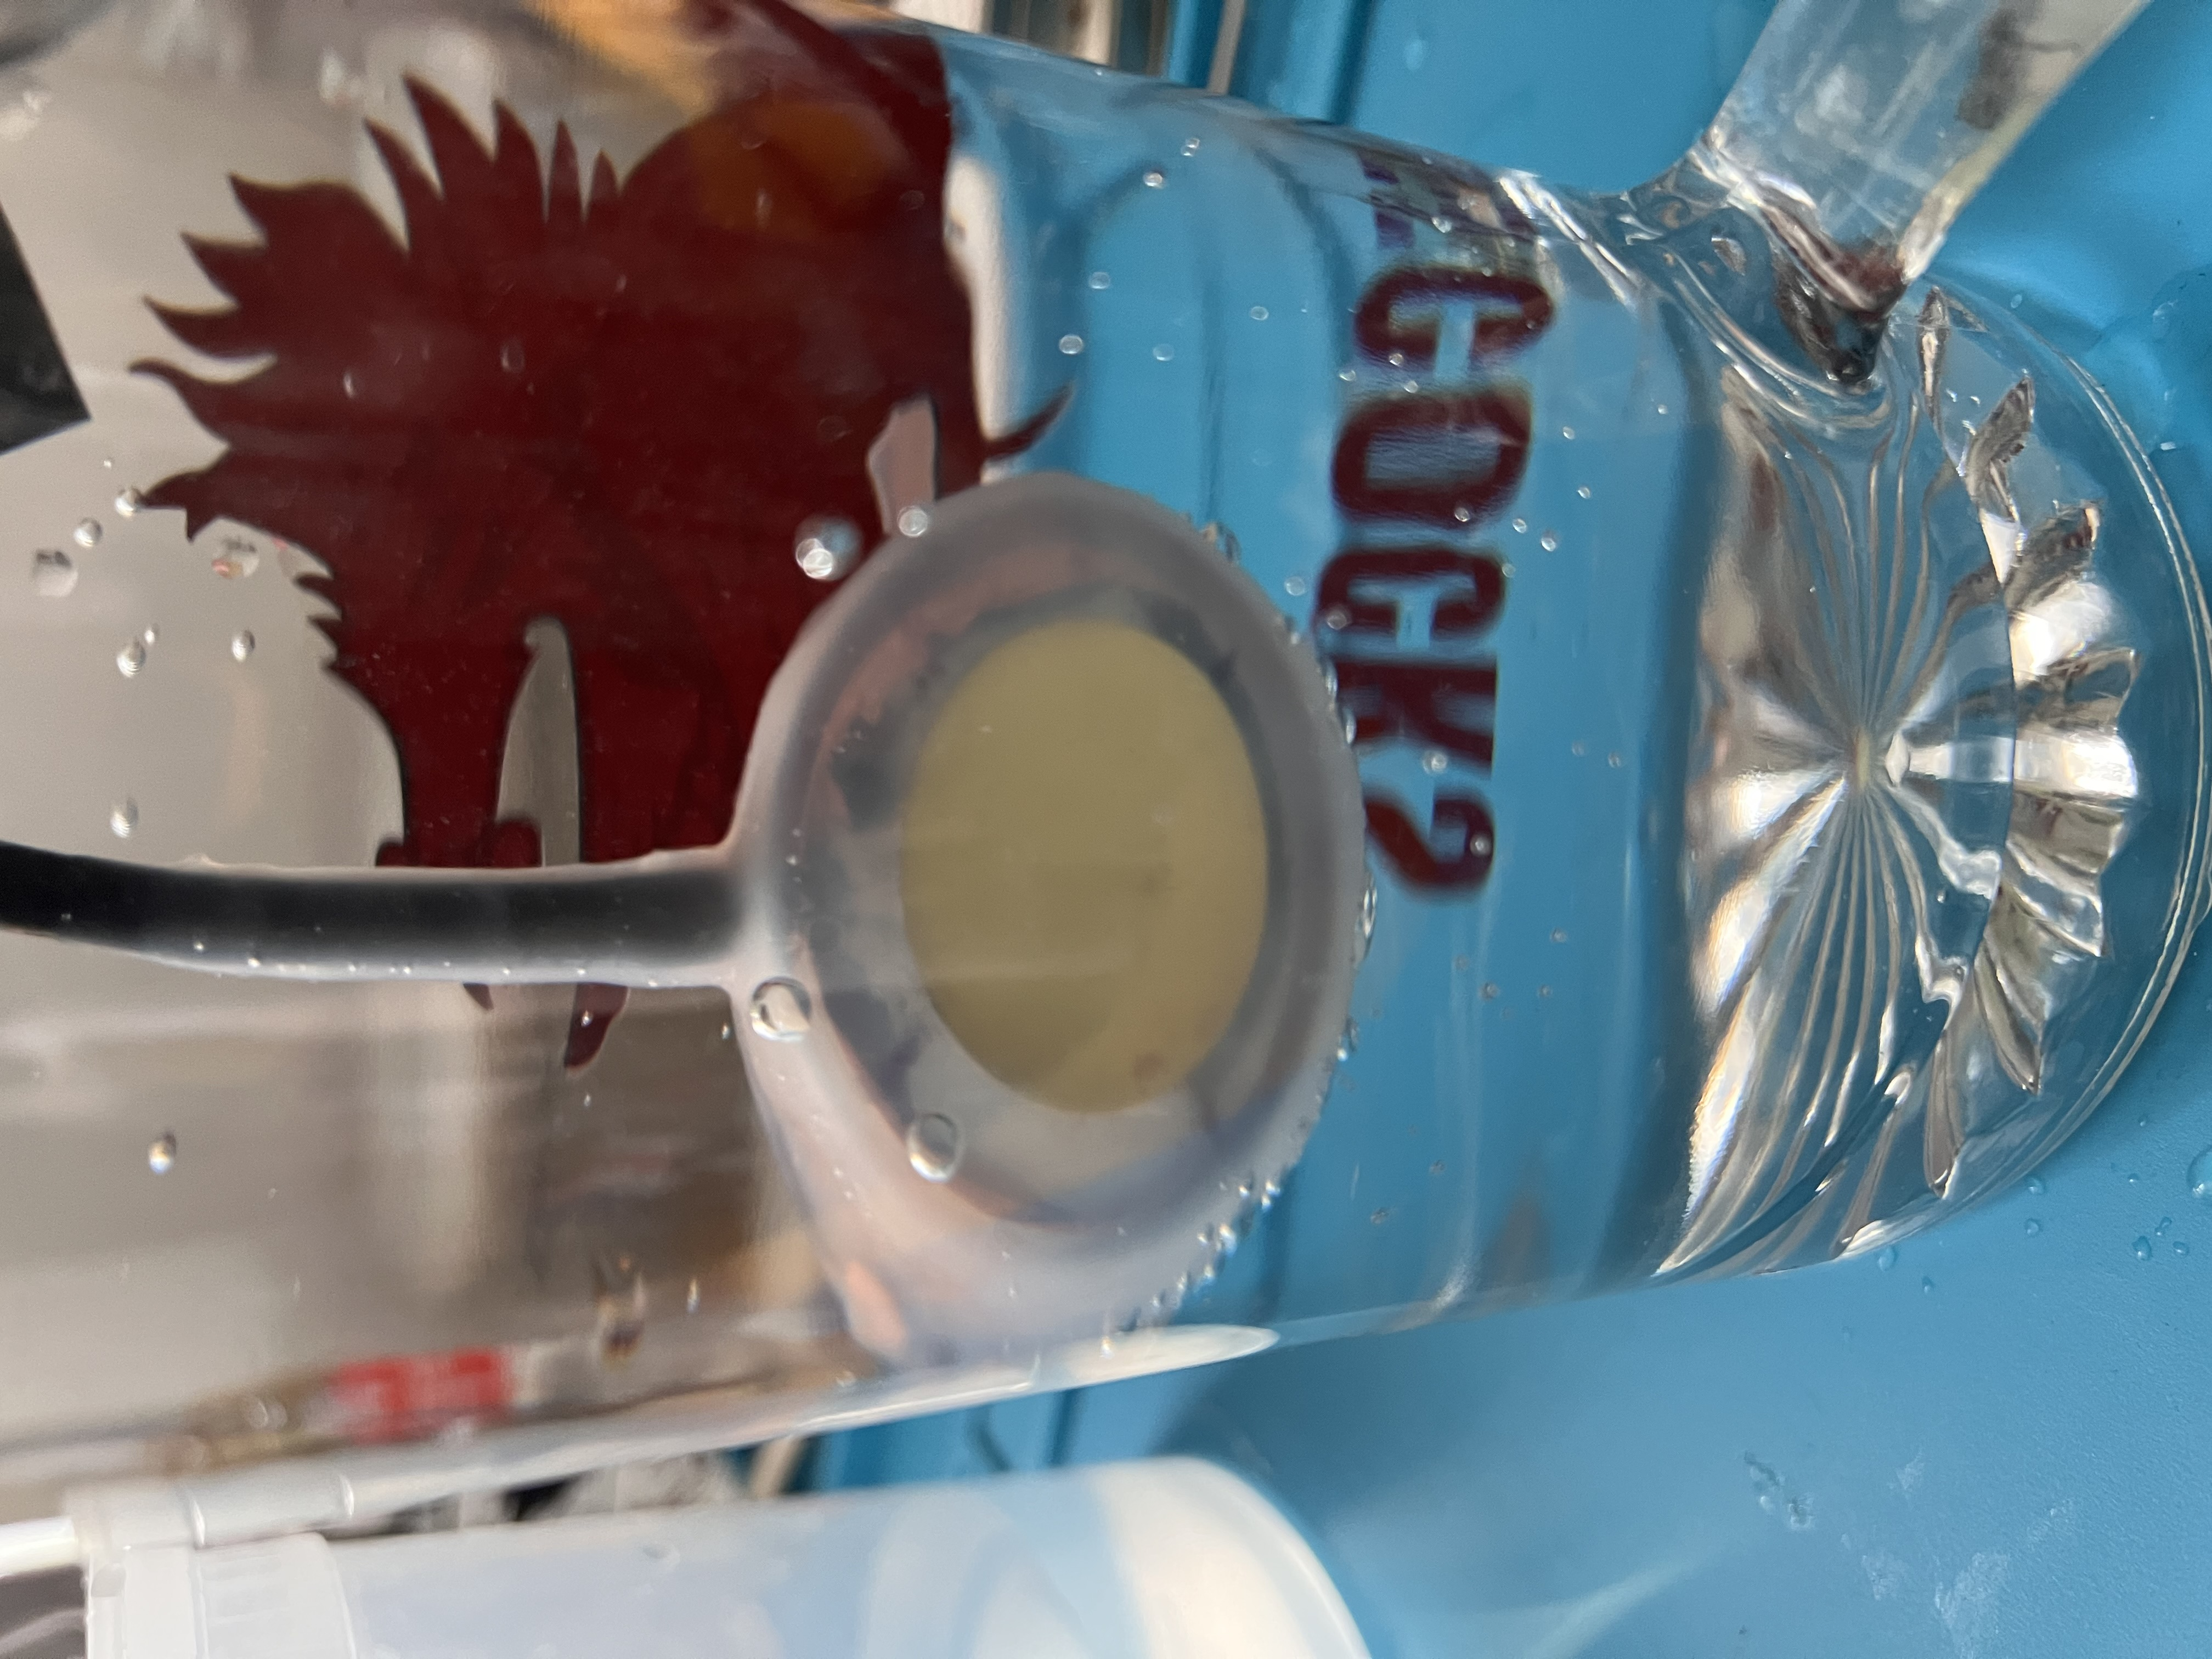
\includegraphics[width=0.31\textwidth]{assets/figures/IMG_6607.jpeg}
	
	\caption{Hydrophones in development. The main purpose of these underwater microphones is to capture the sonic activity of objects dissolving and floating in water, translating material transformation into audible signal.}
	\label{fig:hydrophones}
\end{figure}

The core interaction of \emph{Did Sun Ra Fear Cryosleep?} is a speculative ritual: participants submerge artifacts, small symbolic objects, into a vessel of water. The artifacts' reactions: dissolving, floating, sinking, fragmenting—are captured by hydrophones (underwater microphones) that translate material transformation into sonic signal. Some artifacts dissolve rapidly (like salt tablets, sugar cubes, water-soluble paper), others slowly (certain soils, clays), and others remain suspended in various states of buoyancy (wax). The hope is the hydrophones will pick up the subtle sounds of dissolution: fizzing, crackling, the gentle movement of water displaced by sinking objects, the friction of sediment settling, etc.

These hydrophone recordings are to be processed through a modified Max patcher where I route the signals through some spectral analysis and granular synthesis chains that I have reconfigured to emphasize transient events and textural evolution. Rather than smoothing or "cleaning" the underwater sounds, the modifications amplify their roughness and instability. The hope is for a sonic metaphor of sorts, of bodies in transition, not yet arrived, not fully dissolved. These processed hydrophone signals are then mixed with samples from NASA's data sonification projects—recordings of electromagnetic waves from space, rhythms, solar wind, etc. creating a sonic environment where earthly dissolution and cosmic travel coexist.

The spatialization approach here differs from that of \emph{Buffalo Soldier}. Here, sounds do not move through space in supposed trajectories; instead, they occupy zones that slowly shift and bleed into one another, like fluids mixing. I aim to develop an "encoding system" of sorts that allows sounds to maintain spatial "weight" and "density". Perhaps these parameters can be extracted from othe sensors in the water or from th properties of the materials of the dissolving objects. Heavier sounds (lower frequencies, denser textures) settle toward "lower positions", while lighter sounds (higher frequencies, more granular) float upward. This creates a vertical mix or vertical spatiality informed by the physics of fluid dynamics.

\subsection{Embodied Development: What Has Emerged}

Initially, I conceived the interaction of this work as a straightforward data sonification project: objects in water, hydrophones capture sound, process and spatialize. But during early experiments, I found myself drawn to the act of pouring water into the glass to test the hydrophones. What is submerging objects became a deliberate, ceremonial gesture required for sonic activation? There is something profound about choosing what to submerge, about watching it dissolve or resist dissolution, about witnessing transformation. This led me to frame the interaction not as "input" but as ritual. This way, participants become "witnesses" to a process of passage and transformation.

The choice of artifacts has proven more complex than anticipated. Different materials produce wildly different sonic results and are not as easily captured on hydrophones: effervescent tablets create aggressive, noisy textures; salt dissolves with barely perceptible sound. I have been planning to experimenting with creating custom artifacts. Making molds and using compressed mixtures of materials designed to dissolve at specific rates (sugar, salt, wax, clay/plaster). This moves the work closer to what I think of as kind of "compositional" chemistry, where material properties become compositional parameters. I am also looking into other sensors to incorporate to gather and utilize real-time data of dissolving materials in water. Like, maybe using a sensor to measure the change in conductivity of the solution based on the dissolved materials.

The work continues to evolve. Current explorations include beginning to develop a more sophisticated artifact taxonomy (categorizing materials by dissolution rate, sonic character, symbolic resonance) and refining the vertical spatialization system to better encode the phenomenology of floating and sinking. I am also considering whether the work should include visual projection or light in some way, video of the dissolving artifacts, microscopic views of sediment, archival images of water, images from satellites, etc.

\subsection{ST Domain Integration}

\textbf{Fugitive Speculation (FS):} The work refuses to separate historical trauma (Middle Passage) from speculative futures (interstellar travel), instead insisting on their connection through the figure of the Black body in suspension. By asking whether Sun Ra feared cryosleep, it speculatively centers Black subjectivity within narratives of cosmic passage that typically erase or marginalize it.

\textbf{Material Memory (MM):} Water carries memory. Both as historical archive (the Atlantic) and as material substrate (dissolution, transformation, passage). The ritual of submerging artifacts engages embodied memory of baptism, burial at sea, and other water-based ceremonies. This work also arises from my love and fascination with space and the fact that in many instances, space is depicted as a form of "superfluid." an intimate connection to water.

\textbf{Sensory Worlding (SW):} The work creates a sensory environment organized around fluid dynamics rather than more horizontally aligned terrestrial spatial norms. The vertical spatialization—demands a different mode of listening, one attuned to gradual transformation and spatial weight. The mixing of hydrophone recordings with NASA sonifications creates a sonic world where earthly and cosmic scales interpenetrate.

\textbf{Intimate Witnessing (IW):} The ritual framing positions participants as witnesses rather than users, requiring a different quality of attention and presence. The work's effectiveness depends on whether the sonic transformations evoke the phenomenology of passage, suspension, and dissolution. And whether listeners can sense the connection between dissolving salt and dissolving boundaries, between floating artifacts and floating bodies.